\documentclass[12pt,fleqn]{article}\usepackage{../../common}
\begin{document}
Ay'a Gidelim, K�s�tlanm�� 3-Cisim Problemi (Restricted 3-Body Problem)

spacedyn 704
numcru 133

Newton'un 2. Hareket Kanununu hat�rlarsak vekt�rsel anl�k $\vec{F}$
kuvvetin $m$ k�tlesi �zerinde etkisinin yol a�t��� anl�k y�nsel ivme
$\vec{a}$. 

$$ \vec{F} = m \vec{a} $$

Bir di�er Newton kanunu iki k�tle aras�ndaki kar��l�kl� �ekim kuvveti,

$$ 
|\vec{F}| = G \frac{m_1 m_2}{r^2}
$$

$r$ iki k�tle $m_1,m_2$ aras�ndaki mesafe, basitlik a��s�ndan t�m
k�tlelerinin orta noktalar�na odakl� oldu�u farzedilir. Bu kuvvetin y�nsel
hali i�in $\vec{r}$ y�n�nde birim vekt�r� hesaplar�z, $\vec{r}/|r|$ ve bu
birim vekt�r� �stteki kuvvet ile �arpar�z,

$$ 
F = |\vec{F}| \cdot \frac{\vec{r}}{|r|}  
= G \frac{m_1 m_2}{r^2}\cdot \frac{\vec{r}}{|r|} 
= G \frac{m_1 m_2}{r^3}\cdot \vec{r}
$$









two body, space dyn - 374, 524, 553

szebehely pg 418

analyti-schaub 509





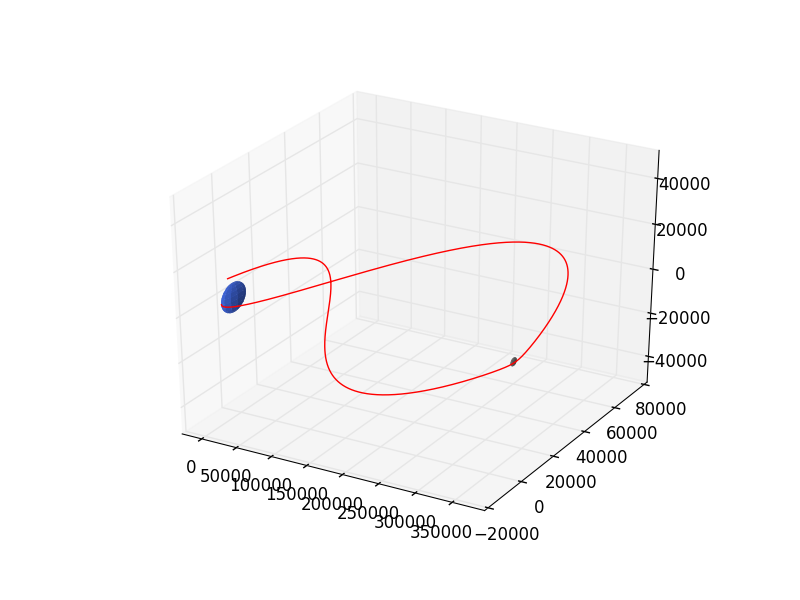
\includegraphics[width=20em]{chaos_app01_01.png}

Kaynaklar

[1] Stack Exchange, {\em Restricted Three-Body Problem}, \url{http://math.stackexchange.com/questions/54735/restricted-three-body-problem}


\end{document}
